% generated by gen_arch_v3.py -- do not edit by hand
\documentclass[10pt]{standalone}
\usepackage{helvet}
\renewcommand{\familydefault}{\sfdefault}
\usepackage{amsmath,amssymb}
\usepackage{tikz}
\usetikzlibrary{arrows.meta}
\definecolor{cstage}{HTML}{FFF8E1}
\definecolor{cctrl}{HTML}{D6E0EC}
\definecolor{cctrlb}{HTML}{3B5675}
\definecolor{cexe}{HTML}{FFE699}
\definecolor{cexeb}{HTML}{7F6000}
\definecolor{cmask}{HTML}{D9EAD3}
\definecolor{cmaskb}{HTML}{38761D}
\definecolor{cmem}{HTML}{F4CCCC}
\definecolor{cmemb}{HTML}{CC0000}
\definecolor{chl}{HTML}{FCE4D6}
\definecolor{chlb}{HTML}{C55A11}
\newcommand{\fs}{\fontsize{6.4}{7.4}\selectfont}
\newcommand{\fss}{\fontsize{5.8}{6.6}\selectfont}
\begin{document}
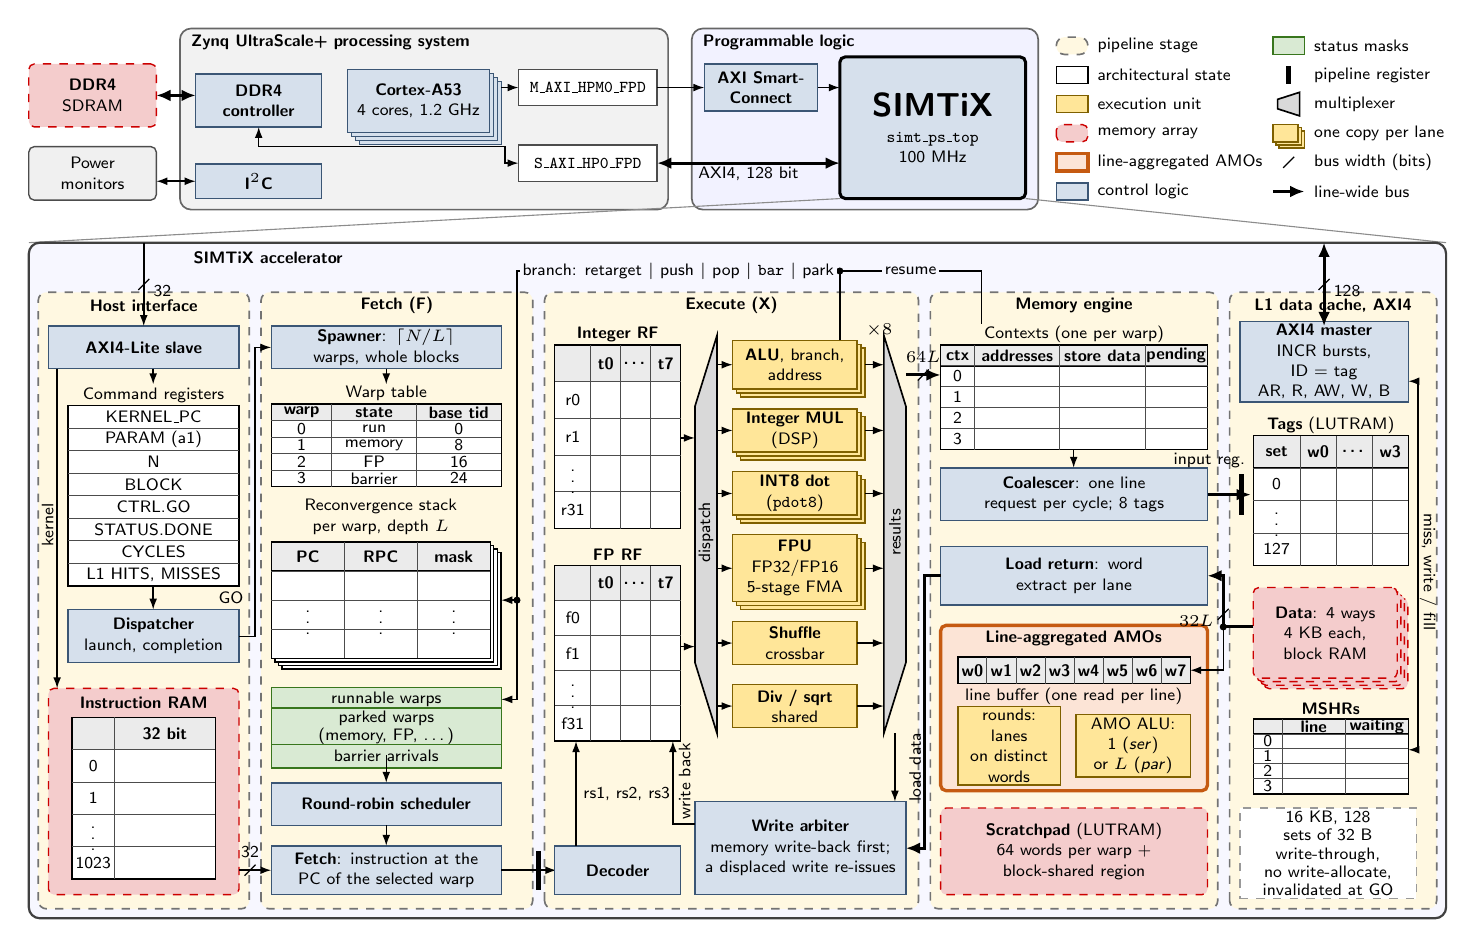
\begin{tikzpicture}[x=1cm, y=1cm,
  base/.style={align=center, font=\fs, inner sep=1pt, line width=0.5pt},
  ctrl/.style={base, draw=cctrlb, fill=cctrl},  ctrlbox/.style={draw=cctrlb, fill=cctrl, line width=0.5pt},
  exe/.style={base, draw=cexeb, fill=cexe},     exebox/.style={draw=cexeb, fill=cexe, line width=0.5pt},
  mask/.style={base, draw=cmaskb, fill=cmask, font=\fss}, maskbox/.style={draw=cmaskb, fill=cmask, line width=0.5pt},
  memarr/.style={base, draw=cmemb, fill=cmem, dashed, rounded corners=2pt},
  memarrbox/.style={draw=cmemb, fill=cmem, dashed, rounded corners=2pt, line width=0.5pt},
  hl/.style={draw=chlb, fill=chl, line width=1.2pt, rounded corners=2pt},
  hlbox/.style={draw=chlb, fill=chl, line width=1.2pt},
  acc/.style={base, draw=black, fill=cctrl, line width=1.1pt, rounded corners=2pt},
  port/.style={base, draw=black!70, fill=white, font=\fss\ttfamily},
  offchip/.style={base, draw=black!70, fill=black!6, rounded corners=2pt},
  note/.style={base, draw=black!40, fill=white, dashed, font=\fss},
  tbl/.style={draw=black, line width=0.5pt}, tblline/.style={draw=black!70, line width=0.35pt},
  cell/.style={font=\fss, inner sep=0.5pt}, cellh/.style={font=\fss\bfseries, inner sep=0.5pt},
  tbltitle/.style={font=\fs, inner sep=0.5pt},
  stagebox/.style={draw=black!55, dashed, fill=cstage, rounded corners=3pt, line width=0.6pt},
  stagetitle/.style={font=\fs\bfseries, inner sep=0.5pt},
  psframe/.style={draw=black!60, fill=black!5, rounded corners=4pt, line width=0.6pt},
  plframe/.style={draw=black!60, fill=blue!5, rounded corners=4pt, line width=0.6pt},
  accframe/.style={draw=black!75, fill=blue!3, rounded corners=4pt, line width=0.8pt},
  paneltitle/.style={font=\fs, inner sep=1pt},
  mux/.style={draw=black, fill=black!15, line width=0.6pt},
  lbl/.style={font=\fs, inner sep=0.5pt},
  elabel/.style={font=\fss, inner sep=1pt},
  wlabel/.style={font=\fss, inner sep=0.5pt},
  keytext/.style={font=\fss, inner sep=0.5pt},
  buslabel/.style={font=\fss, fill=blue!3, inner sep=1pt},
  vlabel/.style={font=\fss, rotate=90, inner sep=0.5pt},
  vlabelr/.style={font=\fss, rotate=-90, inner sep=0.5pt},
  zoom/.style={draw=black!45, line width=0.4pt},
  line/.style={line width=0.55pt},
  arr/.style={-{Latex[length=1.4mm, width=1.0mm]}, line width=0.55pt},
  darr/.style={{Latex[length=1.4mm, width=1.0mm]}-{Latex[length=1.4mm, width=1.0mm]}, line width=0.55pt},
  bus/.style={-{Latex[length=1.8mm, width=1.5mm]}, line width=1.1pt},
  bdarr/.style={{Latex[length=1.8mm, width=1.5mm]}-{Latex[length=1.8mm, width=1.5mm]}, line width=1.1pt}]
\node[memarr, minimum width=1.620cm, minimum height=0.800cm, text width=1.520cm] (ddr) at (0.810,10.450) {\textbf{DDR4}\\SDRAM};
\node[offchip, minimum width=1.620cm, minimum height=0.680cm, text width=1.520cm] (mon) at (0.810,9.460) {Power\\monitors};
\draw[psframe] (1.920,9.000) rectangle (8.120,11.300);
\node[paneltitle, anchor=north west] at (2.020,11.260) {\textbf{Zynq UltraScale+ processing system}};
\node[ctrl, minimum width=1.600cm, minimum height=0.670cm, text width=1.500cm] (ddrc) at (2.920,10.385) {\textbf{DDR4}\\\textbf{controller}};
\node[ctrl, minimum width=1.600cm, minimum height=0.440cm, text width=1.500cm] (i2c) at (2.920,9.360) {\textbf{I$^2$C}};
\draw[ctrlbox] (4.200,9.830) rectangle (6.000,10.630);
\draw[ctrlbox] (4.150,9.880) rectangle (5.950,10.680);
\draw[ctrlbox] (4.100,9.930) rectangle (5.900,10.730);
\node[ctrl, minimum width=1.800cm, minimum height=0.800cm, text width=1.700cm] (a53) at (4.950,10.380) {\textbf{Cortex-A53}\\4 cores, 1.2~GHz};
\node[port, minimum width=1.760cm, minimum height=0.460cm, text width=1.660cm] (hpm) at (7.100,10.550) {M\_AXI\_HPM0\_FPD};
\node[port, minimum width=1.760cm, minimum height=0.460cm, text width=1.660cm] (hp0) at (7.100,9.590) {S\_AXI\_HP0\_FPD};
\draw[arr] (6.000,10.550) -- (6.220,10.550);
\draw[darr] (6.220,9.590) -- (6.050,9.590) -- (6.050,9.800) -- (2.920,9.800) -- (2.920,10.050);
\draw[bdarr] (2.120,10.450) -- (1.620,10.450);
\draw[darr] (2.120,9.360) -- (1.620,9.360);
\draw[plframe] (8.420,9.000) rectangle (12.820,11.300);
\node[paneltitle, anchor=north west] at (8.520,11.260) {\textbf{Programmable logic}};
\node[ctrl, minimum width=1.440cm, minimum height=0.600cm, text width=1.340cm] (sc) at (9.300,10.550) {\textbf{AXI Smart-}\\\textbf{Connect}};
\node[acc, minimum width=2.360cm, minimum height=1.800cm, text width=2.260cm] (simtix) at (11.480,10.040) {\textbf{\large SIMTiX}\\[2pt]\texttt{simt\_ps\_top}\\100~MHz};
\draw[arr] (7.980,10.550) -- (8.580,10.550);
\draw[arr] (10.020,10.550) -- (10.300,10.550);
\draw[bdarr] (10.300,9.590) -- node[elabel, pos=0.5, below] {AXI4, 128 bit} (7.980,9.590);
\draw[stagebox] (13.050,10.970) rectangle (13.450,11.190);
\node[keytext, anchor=west] at (13.550,11.080) {pipeline stage};
\draw[tbl, fill=white] (13.050,10.600) rectangle (13.450,10.820);
\node[keytext, anchor=west] at (13.550,10.710) {architectural state};
\draw[exebox] (13.050,10.230) rectangle (13.450,10.450);
\node[keytext, anchor=west] at (13.550,10.340) {execution unit};
\draw[memarrbox] (13.050,9.860) rectangle (13.450,10.080);
\node[keytext, anchor=west] at (13.550,9.970) {memory array};
\draw[hlbox] (13.050,9.490) rectangle (13.450,9.710);
\node[keytext, anchor=west] at (13.550,9.600) {line-aggregated AMOs};
\draw[ctrlbox] (13.050,9.120) rectangle (13.450,9.340);
\node[keytext, anchor=west] at (13.550,9.230) {control logic};
\draw[maskbox] (15.800,10.970) rectangle (16.200,11.190);
\node[keytext, anchor=west] at (16.300,11.080) {status masks};
\fill[black] (15.965,10.590) rectangle (16.035,10.830);
\node[keytext, anchor=west] at (16.300,10.710) {pipeline register};
\draw[mux] (15.860,10.280) -- (16.140,10.190) -- (16.140,10.490) -- (15.860,10.400) -- cycle;
\node[keytext, anchor=west] at (16.300,10.340) {multiplexer};
\draw[exebox] (15.880,9.780) rectangle (16.200,10.000);
\draw[exebox] (15.840,9.820) rectangle (16.160,10.040);
\draw[exebox] (15.800,9.860) rectangle (16.120,10.080);
\node[keytext, anchor=west] at (16.300,9.970) {one copy per lane};
\draw[line width=0.45pt] (15.93,9.530) -- (16.07,9.670);
\node[keytext, anchor=west] at (16.300,9.600) {bus width (bits)};
\draw[bus] (15.80,9.230) -- (16.20,9.230);
\node[keytext, anchor=west] at (16.300,9.230) {line-wide bus};
\draw[zoom] (10.30,9.14) -- (0.00,8.58);
\draw[zoom] (12.66,9.14) -- (18.00,8.58);
\draw[accframe] (0.000,0.000) rectangle (18.000,8.580);
\node[paneltitle, anchor=north west] at (2.050,8.500) {\textbf{SIMTiX accelerator}};
\draw[stagebox] (0.120,0.120) rectangle (2.800,7.950);
\node[stagetitle, anchor=center] at (1.460,7.780) {Host interface};
\node[ctrl, minimum width=2.420cm, minimum height=0.540cm, text width=2.320cm] (axil) at (1.460,7.250) {\textbf{AXI4-Lite slave}};
\node[tbltitle, anchor=center] at (1.585,6.645) {Command registers};
\draw[tbl, fill=white] (0.500,4.220) rectangle (2.670,6.510);
\draw[tblline] (0.500,6.224) -- (2.670,6.224);
\draw[tblline] (0.500,5.938) -- (2.670,5.938);
\draw[tblline] (0.500,5.651) -- (2.670,5.651);
\draw[tblline] (0.500,5.365) -- (2.670,5.365);
\draw[tblline] (0.500,5.079) -- (2.670,5.079);
\draw[tblline] (0.500,4.792) -- (2.670,4.792);
\draw[tblline] (0.500,4.506) -- (2.670,4.506);
\node[cell, anchor=center] at (1.585,6.367) {KERNEL\_PC};
\node[cell, anchor=center] at (1.585,6.081) {PARAM (a1)};
\node[cell, anchor=center] at (1.585,5.794) {N};
\node[cell, anchor=center] at (1.585,5.508) {BLOCK};
\node[cell, anchor=center] at (1.585,5.222) {CTRL.GO};
\node[cell, anchor=center] at (1.585,4.936) {STATUS.DONE};
\node[cell, anchor=center] at (1.585,4.649) {CYCLES};
\node[cell, anchor=center] at (1.585,4.363) {L1 HITS, MISSES};
\node[ctrl, minimum width=2.170cm, minimum height=0.670cm, text width=2.070cm] (disp) at (1.585,3.585) {\textbf{Dispatcher}\\launch, completion};
\draw[memarr] (0.250,0.300) rectangle (2.670,2.920);
\node[tbltitle, anchor=center] at (1.460,2.740) {\textbf{Instruction RAM}};
\draw[tbl, fill=white] (0.550,0.500) rectangle (2.370,2.550);
\draw[tbl, fill=black!8] (0.550,2.140) rectangle (2.370,2.550);
\draw[tblline] (0.550,2.140) -- (2.370,2.140);
\draw[tblline] (0.550,1.730) -- (2.370,1.730);
\draw[tblline] (0.550,1.320) -- (2.370,1.320);
\draw[tblline] (0.550,0.910) -- (2.370,0.910);
\draw[tblline] (1.085,0.500) -- (1.085,2.550);
\node[cellh, anchor=center] at (1.728,2.345) {32 bit};
\node[cell, anchor=center] at (0.818,1.935) {0};
\node[cell, anchor=center] at (0.818,1.525) {1};
\node[cell, anchor=center] at (0.818,1.115) {$\vdots$};
\node[cell, anchor=center] at (0.818,0.705) {1023};
\draw[arr] (1.460,8.580) -- (1.460,7.520);
\draw[line width=0.45pt] (1.390,7.980) -- (1.530,8.120);
\node[wlabel, anchor=west] at (1.560,7.970) {32};
\draw[arr] (1.580,6.980) -- (1.580,6.780);
\draw[arr] (0.360,6.980) -- (0.360,2.920);
\node[vlabel, anchor=center] at (0.240,5.000) {kernel};
\draw[arr] (1.580,4.220) -- (1.580,3.920);
\draw[stagebox] (2.950,0.120) rectangle (6.400,7.950);
\node[stagetitle, anchor=center] at (4.675,7.780) {Fetch (F)};
\node[ctrl, minimum width=2.920cm, minimum height=0.540cm, text width=2.820cm] (spawn) at (4.540,7.250) {\textbf{Spawner}: $\lceil N/L\rceil$ warps, whole blocks};
\node[tbltitle, anchor=center] at (4.540,6.665) {Warp table};
\draw[tbl, fill=white] (3.080,5.480) rectangle (6.000,6.530);
\draw[tbl, fill=black!8] (3.080,6.320) rectangle (6.000,6.530);
\draw[tblline] (3.080,6.320) -- (6.000,6.320);
\draw[tblline] (3.080,6.110) -- (6.000,6.110);
\draw[tblline] (3.080,5.900) -- (6.000,5.900);
\draw[tblline] (3.080,5.690) -- (6.000,5.690);
\draw[tblline] (3.848,5.480) -- (3.848,6.530);
\draw[tblline] (4.924,5.480) -- (4.924,6.530);
\node[cellh, anchor=center] at (3.464,6.425) {warp};
\node[cellh, anchor=center] at (4.386,6.425) {state};
\node[cellh, anchor=center] at (5.462,6.425) {base tid};
\node[cell, anchor=center] at (3.464,6.215) {0};
\node[cell, anchor=center] at (4.386,6.215) {run};
\node[cell, anchor=center] at (5.462,6.215) {0};
\node[cell, anchor=center] at (3.464,6.005) {1};
\node[cell, anchor=center] at (4.386,6.005) {memory};
\node[cell, anchor=center] at (5.462,6.005) {8};
\node[cell, anchor=center] at (3.464,5.795) {2};
\node[cell, anchor=center] at (4.386,5.795) {FP};
\node[cell, anchor=center] at (5.462,5.795) {16};
\node[cell, anchor=center] at (3.464,5.585) {3};
\node[cell, anchor=center] at (4.386,5.585) {barrier};
\node[cell, anchor=center] at (5.462,5.585) {24};
\draw[tbl, fill=white] (3.215,3.165) rectangle (5.995,4.645);
\draw[tbl, fill=white] (3.170,3.210) rectangle (5.950,4.690);
\draw[tbl, fill=white] (3.125,3.255) rectangle (5.905,4.735);
\draw[tbl, fill=white] (3.080,3.300) rectangle (5.860,4.780);
\draw[tbl, fill=black!8] (3.080,4.410) rectangle (5.860,4.780);
\draw[tblline] (3.080,4.410) -- (5.860,4.410);
\draw[tblline] (3.080,4.040) -- (5.860,4.040);
\draw[tblline] (3.080,3.670) -- (5.860,3.670);
\draw[tblline] (4.007,3.300) -- (4.007,4.780);
\draw[tblline] (4.933,3.300) -- (4.933,4.780);
\node[cellh, anchor=center] at (3.543,4.595) {PC};
\node[cellh, anchor=center] at (4.470,4.595) {RPC};
\node[cellh, anchor=center] at (5.397,4.595) {mask};
\node[cell, anchor=center] at (3.543,3.855) {$\vdots$};
\node[cell, anchor=center] at (4.470,3.855) {$\vdots$};
\node[cell, anchor=center] at (5.397,3.855) {$\vdots$};
\node[tbltitle, align=center] at (4.47,5.10) {Reconvergence stack\\per warp, depth $L$};
\node[mask, minimum width=2.920cm, minimum height=0.300cm, text width=2.820cm] (m0) at (4.540,2.780) {runnable warps};
\node[mask, minimum width=2.920cm, minimum height=0.300cm, text width=2.820cm] (m1) at (4.540,2.420) {parked warps (memory, FP, \ldots)};
\node[mask, minimum width=2.920cm, minimum height=0.300cm, text width=2.820cm] (m2) at (4.540,2.060) {barrier arrivals};
\node[ctrl, minimum width=2.920cm, minimum height=0.540cm, text width=2.820cm] (sched) at (4.540,1.450) {\textbf{Round-robin scheduler}};
\node[ctrl, minimum width=2.920cm, minimum height=0.620cm, text width=2.820cm] (fetch) at (4.540,0.610) {\textbf{Fetch}: instruction at the\\PC of the selected warp};
\draw[arr] (4.540,6.980) -- (4.540,6.780);
\draw[arr] (4.540,2.070) -- (4.540,1.720);
\draw[arr] (4.540,1.180) -- (4.540,0.920);
\draw[arr] (2.670,3.580) -- (2.875,3.580) -- (2.875,7.250) -- (3.080,7.250);
\node[wlabel, anchor=east] at (2.750,4.070) {GO};
\draw[arr] (2.670,0.610) -- (3.080,0.610);
\draw[line width=0.45pt] (2.740,0.540) -- (2.880,0.680);
\node[wlabel, anchor=south] at (2.810,0.750) {32};
\draw[stagebox] (6.550,0.120) rectangle (11.300,7.950);
\node[stagetitle, anchor=center] at (8.925,7.780) {Execute (X)};
\fill[black] (6.440,0.360) rectangle (6.510,0.860);
\draw[arr] (6.000,0.610) -- (6.700,0.610);
\node[tbltitle, anchor=center] at (7.480,7.415) {\textbf{Integer RF}};
\draw[tbl, fill=white] (6.680,4.950) rectangle (8.280,7.280);
\draw[tbl, fill=black!8] (6.680,6.814) rectangle (8.280,7.280);
\draw[tblline] (6.680,6.814) -- (8.280,6.814);
\draw[tblline] (6.680,6.348) -- (8.280,6.348);
\draw[tblline] (6.680,5.882) -- (8.280,5.882);
\draw[tblline] (6.680,5.416) -- (8.280,5.416);
\draw[tblline] (7.137,4.950) -- (7.137,7.280);
\draw[tblline] (7.518,4.950) -- (7.518,7.280);
\draw[tblline] (7.899,4.950) -- (7.899,7.280);
\node[cellh, anchor=center] at (7.328,7.047) {t0};
\node[cellh, anchor=center] at (7.709,7.047) {\ldots};
\node[cellh, anchor=center] at (8.090,7.047) {t7};
\node[cell, anchor=center] at (6.909,6.581) {r0};
\node[cell, anchor=center] at (6.909,6.115) {r1};
\node[cell, anchor=center] at (6.909,5.649) {$\vdots$};
\node[cell, anchor=center] at (6.909,5.183) {r31};
\node[tbltitle, anchor=center] at (7.480,4.615) {\textbf{FP RF}};
\draw[tbl, fill=white] (6.680,2.250) rectangle (8.280,4.480);
\draw[tbl, fill=black!8] (6.680,4.034) rectangle (8.280,4.480);
\draw[tblline] (6.680,4.034) -- (8.280,4.034);
\draw[tblline] (6.680,3.588) -- (8.280,3.588);
\draw[tblline] (6.680,3.142) -- (8.280,3.142);
\draw[tblline] (6.680,2.696) -- (8.280,2.696);
\draw[tblline] (7.137,2.250) -- (7.137,4.480);
\draw[tblline] (7.518,2.250) -- (7.518,4.480);
\draw[tblline] (7.899,2.250) -- (7.899,4.480);
\node[cellh, anchor=center] at (7.328,4.257) {t0};
\node[cellh, anchor=center] at (7.709,4.257) {\ldots};
\node[cellh, anchor=center] at (8.090,4.257) {t7};
\node[cell, anchor=center] at (6.909,3.811) {f0};
\node[cell, anchor=center] at (6.909,3.365) {f1};
\node[cell, anchor=center] at (6.909,2.919) {$\vdots$};
\node[cell, anchor=center] at (6.909,2.473) {f31};
\node[ctrl, minimum width=1.600cm, minimum height=0.620cm, text width=1.500cm] (dec) at (7.480,0.610) {\textbf{Decoder}};
\draw[arr] (6.950,0.920) -- (6.950,2.250);
\node[wlabel, anchor=west] at (7.020,1.580) {rs1, rs2, rs3};
\draw[mux] (8.460,3.250) -- (8.740,2.350) -- (8.740,7.400) -- (8.460,6.500) -- cycle;
\node[vlabel, anchor=center] at (8.600,4.900) {dispatch};
\draw[arr] (8.280,6.100) -- (8.460,6.100);
\draw[arr] (8.280,3.450) -- (8.460,3.450);
\draw[exebox] (9.040,6.620) rectangle (10.620,7.240);
\draw[exebox] (8.990,6.670) rectangle (10.570,7.290);
\node[exe, minimum width=1.580cm, minimum height=0.620cm, text width=1.480cm] (alu) at (9.730,7.030) {\textbf{ALU}, branch,\\address};
\draw[arr] (8.740,7.030) -- (8.940,7.030);
\draw[arr] (10.620,7.030) -- (10.860,7.030);
\draw[exebox] (9.040,5.820) rectangle (10.620,6.370);
\draw[exebox] (8.990,5.870) rectangle (10.570,6.420);
\node[exe, minimum width=1.580cm, minimum height=0.550cm, text width=1.480cm] (mul) at (9.730,6.195) {\textbf{Integer MUL}\\(DSP)};
\draw[arr] (8.740,6.195) -- (8.940,6.195);
\draw[arr] (10.620,6.195) -- (10.860,6.195);
\draw[exebox] (9.040,5.020) rectangle (10.620,5.570);
\draw[exebox] (8.990,5.070) rectangle (10.570,5.620);
\node[exe, minimum width=1.580cm, minimum height=0.550cm, text width=1.480cm] (dot) at (9.730,5.395) {\textbf{INT8 dot}\\(\texttt{pdot8})};
\draw[arr] (8.740,5.395) -- (8.940,5.395);
\draw[arr] (10.620,5.395) -- (10.860,5.395);
\draw[exebox] (9.040,3.920) rectangle (10.620,4.770);
\draw[exebox] (8.990,3.970) rectangle (10.570,4.820);
\node[exe, minimum width=1.580cm, minimum height=0.850cm, text width=1.480cm] (fpu) at (9.730,4.445) {\textbf{FPU}\\FP32/FP16\\5-stage FMA};
\draw[arr] (8.740,4.445) -- (8.940,4.445);
\draw[arr] (10.620,4.445) -- (10.860,4.445);
\node[exe, minimum width=1.580cm, minimum height=0.550cm, text width=1.480cm] (shf) at (9.730,3.495) {\textbf{Shuffle}\\crossbar};
\draw[arr] (8.740,3.495) -- (8.940,3.495);
\draw[arr] (10.520,3.495) -- (10.860,3.495);
\node[exe, minimum width=1.580cm, minimum height=0.550cm, text width=1.480cm] (sfu) at (9.730,2.695) {\textbf{Div / sqrt}\\shared};
\draw[arr] (8.740,2.695) -- (8.940,2.695);
\draw[arr] (10.520,2.695) -- (10.860,2.695);
\node[wlabel, anchor=center] at (10.800,7.470) {$\times 8$};
\draw[mux] (10.860,2.350) -- (11.140,3.250) -- (11.140,6.500) -- (10.860,7.400) -- cycle;
\node[vlabel, anchor=center] at (11.000,4.900) {results};
\node[ctrl, minimum width=2.680cm, minimum height=1.180cm, text width=2.580cm] (arb) at (9.800,0.890) {\textbf{Write arbiter}\\memory write-back first;\\a displaced write re-issues};
\draw[arr] (11.000,2.350) -- (11.000,1.480);
\draw[arr] (8.460,1.200) -- (8.180,1.200) -- (8.180,2.250);
\node[vlabel, anchor=center] at (8.330,1.740) {write back};
\draw[stagebox] (11.450,0.120) rectangle (15.100,7.950);
\node[stagetitle, anchor=center] at (13.275,7.780) {Memory engine};
\node[tbltitle, anchor=center] at (13.275,7.415) {Contexts (one per warp)};
\draw[tbl, fill=white] (11.580,5.950) rectangle (14.970,7.280);
\draw[tbl, fill=black!8] (11.580,7.014) rectangle (14.970,7.280);
\draw[tblline] (11.580,7.014) -- (14.970,7.014);
\draw[tblline] (11.580,6.748) -- (14.970,6.748);
\draw[tblline] (11.580,6.482) -- (14.970,6.482);
\draw[tblline] (11.580,6.216) -- (14.970,6.216);
\draw[tblline] (12.013,5.950) -- (12.013,7.280);
\draw[tblline] (13.095,5.950) -- (13.095,7.280);
\draw[tblline] (14.177,5.950) -- (14.177,7.280);
\node[cellh, anchor=center] at (11.796,7.147) {ctx};
\node[cellh, anchor=center] at (12.554,7.147) {addresses};
\node[cellh, anchor=center] at (13.636,7.147) {store data};
\node[cellh, anchor=center] at (14.573,7.147) {pending};
\node[cell, anchor=center] at (11.796,6.881) {0};
\node[cell, anchor=center] at (11.796,6.615) {1};
\node[cell, anchor=center] at (11.796,6.349) {2};
\node[cell, anchor=center] at (11.796,6.083) {3};
\draw[bus] (11.140,6.900) -- (11.580,6.900);
\draw[line width=0.45pt] (11.290,6.830) -- (11.430,6.970);
\node[wlabel, anchor=south] at (11.360,7.040) {$64L$};
\node[ctrl, minimum width=3.390cm, minimum height=0.670cm, text width=3.290cm] (coal) at (13.275,5.385) {\textbf{Coalescer}: one line\\request per cycle; 8 tags};
\draw[arr] (13.270,5.950) -- (13.270,5.720);
\node[ctrl, minimum width=3.390cm, minimum height=0.740cm, text width=3.290cm] (ldret) at (13.275,4.350) {\textbf{Load return}: word extract per lane};
\draw[hl] (11.580,1.620) rectangle (14.970,3.720);
\node[tbltitle, anchor=center] at (13.270,3.560) {\textbf{Line-aggregated AMOs}};
\draw[tbl, fill=white] (11.800,2.980) rectangle (14.750,3.320);
\draw[tbl, fill=black!8] (11.800,2.980) rectangle (14.750,3.320);
\draw[tblline] (12.169,2.980) -- (12.169,3.320);
\draw[tblline] (12.538,2.980) -- (12.538,3.320);
\draw[tblline] (12.906,2.980) -- (12.906,3.320);
\draw[tblline] (13.275,2.980) -- (13.275,3.320);
\draw[tblline] (13.644,2.980) -- (13.644,3.320);
\draw[tblline] (14.013,2.980) -- (14.013,3.320);
\draw[tblline] (14.381,2.980) -- (14.381,3.320);
\node[cellh, anchor=center] at (11.984,3.150) {w0};
\node[cellh, anchor=center] at (12.353,3.150) {w1};
\node[cellh, anchor=center] at (12.722,3.150) {w2};
\node[cellh, anchor=center] at (13.091,3.150) {w3};
\node[cellh, anchor=center] at (13.459,3.150) {w4};
\node[cellh, anchor=center] at (13.828,3.150) {w5};
\node[cellh, anchor=center] at (14.197,3.150) {w6};
\node[cellh, anchor=center] at (14.566,3.150) {w7};
\node[cell, anchor=center] at (13.270,2.820) {line buffer (one read per line)};
\node[exe, minimum width=1.300cm, minimum height=0.780cm, text width=1.200cm] (rnd) at (12.450,2.190) {rounds: lanes\\on distinct words};
\node[exe, minimum width=1.450cm, minimum height=0.780cm, text width=1.350cm] (aalu) at (14.025,2.190) {AMO ALU: 1 (\emph{ser})\\or $L$ (\emph{par})};
\node[memarr, minimum width=3.390cm, minimum height=1.100cm, text width=3.290cm] (scr) at (13.275,0.850) {\textbf{Scratchpad} (LUTRAM)\\64 words per warp + block-shared region};
\draw[bus] (11.580,4.350) -- (11.370,4.350) -- (11.370,0.890) -- (11.140,0.890);
\node[vlabel, anchor=center] at (11.255,1.920) {load data};
\draw[arr] (12.100,7.550) -- (12.100,8.220) -- (6.200,8.220) -- (6.200,2.780) -- (6.000,2.780);
\draw[line] (10.300,7.340) -- (10.300,8.220);
\fill (10.300,8.220) circle (0.045);
\fill (6.200,4.040) circle (0.045);
\draw[arr] (6.200,4.040) -- (6.000,4.040);
\node[buslabel, anchor=center] at (8.250,8.220) {branch: retarget $\mid$ push $\mid$ pop $\mid$ \texttt{bar} $\mid$ park};
\node[buslabel, anchor=center] at (11.200,8.220) {resume};
\draw[stagebox] (15.250,0.120) rectangle (17.880,7.950);
\node[stagetitle, anchor=center] at (16.565,7.780) {L1 data cache, AXI4};
\node[ctrl, minimum width=2.140cm, minimum height=0.900cm, text width=2.040cm] (axi) at (16.450,7.070) {\textbf{AXI4 master}\\INCR bursts, ID = tag\\AR, R, AW, W, B};
\draw[bdarr] (16.450,7.520) -- (16.450,8.580);
\draw[line width=0.45pt] (16.380,7.980) -- (16.520,8.120);
\node[wlabel, anchor=west] at (16.550,7.970) {128};
\draw[bus] (14.970,5.380) -- (15.520,5.380);
\fill[black] (15.365,5.120) rectangle (15.435,5.640);
\node[wlabel, anchor=east] at (15.470,5.820) {input reg.};
\node[tbltitle, anchor=center] at (16.535,6.265) {\textbf{Tags} (LUTRAM)};
\draw[tbl, fill=white] (15.550,4.480) rectangle (17.520,6.130);
\draw[tbl, fill=black!8] (15.550,5.718) rectangle (17.520,6.130);
\draw[tblline] (15.550,5.718) -- (17.520,5.718);
\draw[tblline] (15.550,5.305) -- (17.520,5.305);
\draw[tblline] (15.550,4.893) -- (17.520,4.893);
\draw[tblline] (16.146,4.480) -- (16.146,6.130);
\draw[tblline] (16.604,4.480) -- (16.604,6.130);
\draw[tblline] (17.062,4.480) -- (17.062,6.130);
\node[cellh, anchor=center] at (15.848,5.924) {set};
\node[cellh, anchor=center] at (16.375,5.924) {w0};
\node[cellh, anchor=center] at (16.833,5.924) {\ldots};
\node[cellh, anchor=center] at (17.291,5.924) {w3};
\node[cell, anchor=center] at (15.848,5.511) {0};
\node[cell, anchor=center] at (15.848,5.099) {$\vdots$};
\node[cell, anchor=center] at (15.848,4.686) {127};
\draw[memarrbox] (15.685,2.915) rectangle (17.515,4.065);
\draw[memarrbox] (15.640,2.960) rectangle (17.470,4.110);
\draw[memarrbox] (15.595,3.005) rectangle (17.425,4.155);
\node[memarr, minimum width=1.830cm, minimum height=1.150cm, text width=1.730cm] (data) at (16.465,3.625) {\textbf{Data}: 4 ways\\4 KB each, block RAM};
\node[tbltitle, anchor=center] at (16.535,2.665) {\textbf{MSHRs}};
\draw[tbl, fill=white] (15.550,1.580) rectangle (17.520,2.530);
\draw[tbl, fill=black!8] (15.550,2.340) rectangle (17.520,2.530);
\draw[tblline] (15.550,2.340) -- (17.520,2.340);
\draw[tblline] (15.550,2.150) -- (17.520,2.150);
\draw[tblline] (15.550,1.960) -- (17.520,1.960);
\draw[tblline] (15.550,1.770) -- (17.520,1.770);
\draw[tblline] (15.919,1.580) -- (15.919,2.530);
\draw[tblline] (16.720,1.580) -- (16.720,2.530);
\node[cellh, anchor=center] at (16.320,2.435) {line};
\node[cellh, anchor=center] at (17.120,2.435) {waiting};
\node[cell, anchor=center] at (15.735,2.245) {0};
\node[cell, anchor=center] at (15.735,2.055) {1};
\node[cell, anchor=center] at (15.735,1.865) {2};
\node[cell, anchor=center] at (15.735,1.675) {3};
\node[note, minimum width=2.240cm, minimum height=1.150cm, text width=2.140cm] (l1note) at (16.500,0.825) {16~KB, 128 sets of 32~B\\write-through,\\no write-allocate,\\invalidated at GO};
\draw[darr] (17.520,2.140) -- (17.640,2.140) -- (17.640,6.820) -- (17.520,6.820);
\node[vlabelr, anchor=center] at (17.770,4.400) {miss, write / fill};
\draw[bus] (15.550,3.700) -- (15.170,3.700) -- (15.170,4.350) -- (14.970,4.350);
\fill (15.170,3.700) circle (0.045);
\draw[arr] (15.170,3.700) -- (15.170,3.150) -- (14.750,3.150);
\draw[line width=0.45pt] (15.100,3.790) -- (15.240,3.930);
\node[wlabel, anchor=east] at (15.070,3.780) {$32L$};
\end{tikzpicture}
\end{document}
